\headline{{\textbf{\Large\sffamily Bonsai Roots:}}\\
          {\textbf{\large\sffamily Meet the Members of TWBC}}}
\label{2025-12-roots}
\noindent
In every edition of \emph{Bonsai Roots}, we pause from wiring, watering, and weekend workshops to celebrate the people who shape our club.
Each story adds character to the ever\--growing forest of TWBC\@.
This month, we are delighted to introduce a member with a wealth of experience and a lifelong connection to his trees: \textbf{Rob Stewart}!

\begin{itemize}
    \item \textbf{What's your name and where in the country do you live?}

    \emph{My name is Rob Stewart, and I am based locally in Isleworth. It is a great spot to be for a bonsai enthusiast, with plenty of inspiration nearby.}

    \item \textbf{What are your favourite species of tree and why?}

    \emph{I have always had a soft spot for Maples. There is something truly magical about the way they transition through the seasons, but it is those vibrant, fiery autumn colours that really seal the deal for me.}

    \item \textbf{What aspect of bonsai do you enjoy?}

    \emph{The hands-on work is what I find most rewarding. I particularly enjoy the technical side of the hobby---pruning and shaping the branches to find the hidden form within the tree.}

    \item \textbf{What aspects of bonsai do you find most challenging?}

    \emph{Pines, without a doubt! They have their own set of rules and a specific rhythm that can be quite demanding to master, even after many years of practice.}

    \begin{window}[2,l,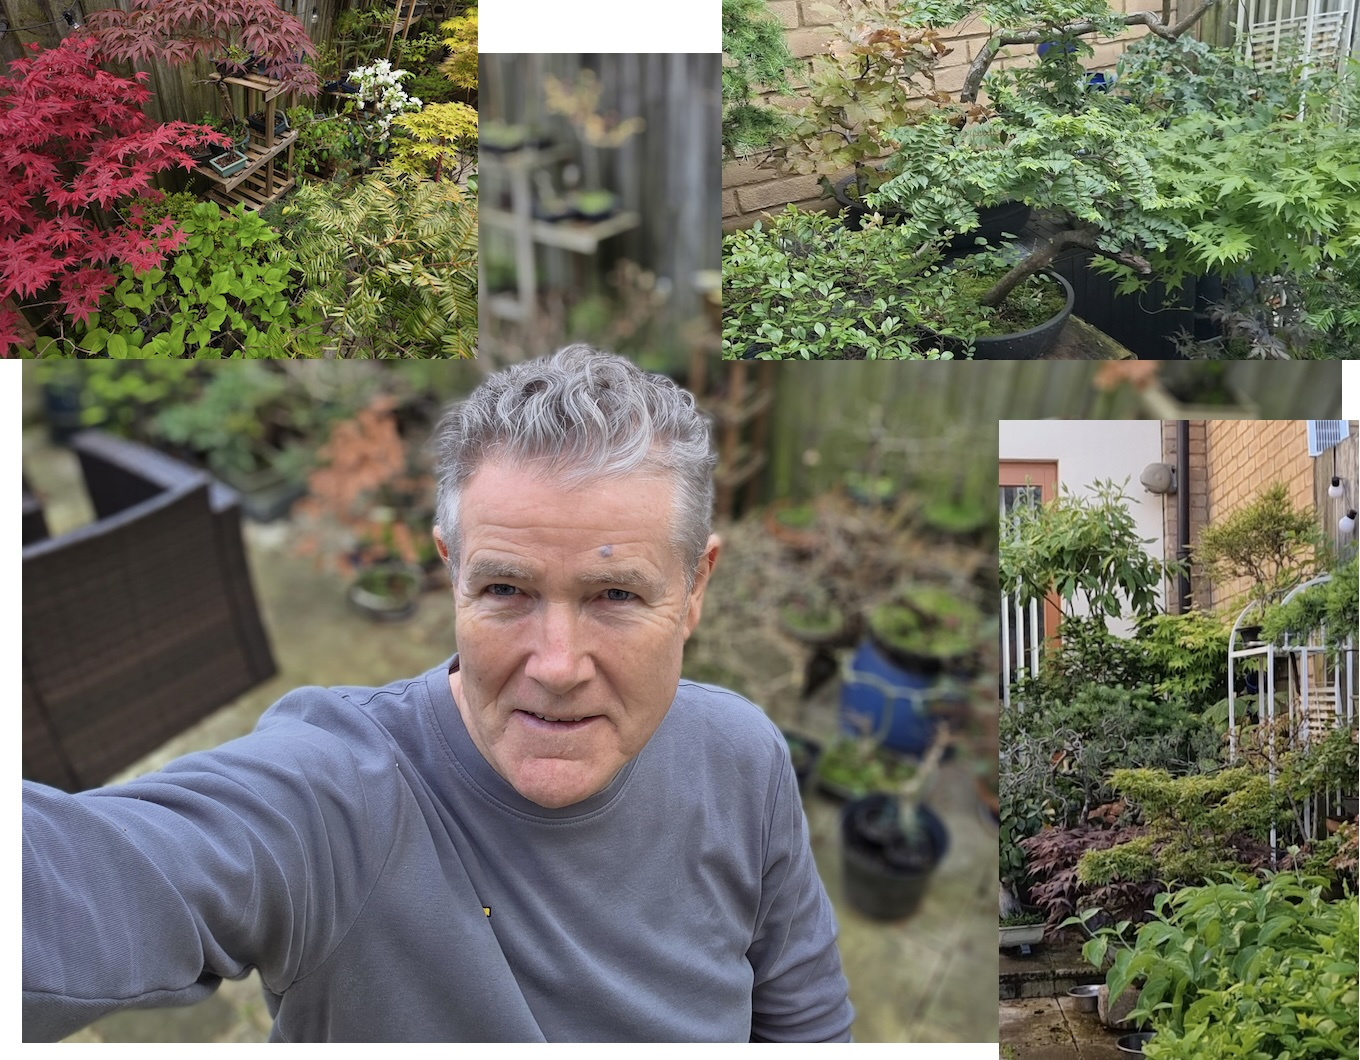
\includegraphics[width=1.0\columnwidth]{2025_12/res/roots_rob_stewart},\centerline{\emph{Rob in his garden with some of his long-term bonsai friends.}}]
    \end{window}
    \columnbreak

    \item \textbf{Who or what inspires you throughout your bonsai journey?}

    \emph{For me, it is the trees themselves. They aren't just plants to me; they are like family. Watching them grow and change over the decades provides all the inspiration I need.}

    \item \textbf{How long have you been interested in keeping bonsai?}

    \emph{It has been a long-term passion of mine. I have been interested in and keeping bonsai for over 30 years now, so they have seen me through many different stages of life.}

    \item \textbf{What stimulated your interest in bonsai?}

    \emph{My interest actually began during my time in the Royal Navy. It was a unique environment to start a hobby, but the discipline and patience of the craft really resonated with me back then.}

    \item \textbf{If you could give someone new to bonsai any tips, what would it be?}

    \emph{It is quite simple: if you have a genuine love for nature, you will naturally fall in love with these small trees. Just lean into that appreciation for the natural world.}

    \item \textbf{Why do you enjoy being part of TWBC, and do you have any ideas or suggestions for the club's future?}

    \emph{The best part of being a member here is the community. Having the opportunity for consistent advice and guidance from fellow enthusiasts is absolutely invaluable.}

    \item \textbf{One word to describe what bonsai means to you?}

    \emph{Companionship. They have always travelled with me through life; they truly are part of the family.}

    \item \textbf{What are your future goals regarding your own trees and learning more about the hobby?}

    \emph{I'm currently focused on refinement. My main goal is to get all of my trees looking top-notch and reaching their full aesthetic potential.}

    \item \textbf{How would you like to see your bonsai journey progress in the future?}

    \emph{On a practical note, I am looking forward to simply having enough time to get all my repotting done in the spring! It’s a busy time, but a very rewarding one.}
\end{itemize}

Rob’s journey is a testament to the lifelong bond we form with our trees---a story of travel, service, and a deep-rooted love for nature.
We are lucky to have his experience in the club.
Who will we meet next time?
Stay tuned for more in \emph{Bonsai Roots}!

\begin{center}
$\cdots$
\end{center}

\noindent
\emph{If you're a newer member and would like to feature in a future edition of Bonsai Roots, simply fill out the form at \href{https://forms.gle/quVXa4L8rhpnT5kr6}{this link}! We'd love to hear your story.}

\closearticle
\columnbreak